\documentclass{article}

% if you need to pass options to natbib, use, e.g.:
%     \PassOptionsToPackage{numbers, compress}{natbib}
% before loading neurips_2024

% ready for submission
\usepackage[preprint]{neurips_2024}

\usepackage[utf8]{inputenc}
\usepackage[T1]{fontenc}
\usepackage{hyperref}
\usepackage{url}
\usepackage{booktabs}
\usepackage{amsfonts}
\usepackage{nicefrac}
\usepackage{microtype}
\usepackage{xcolor}
\usepackage{graphicx}
\usepackage{amsmath}
\usepackage{amssymb}

\title{Detecting Information Cascades in Polymarket Order Books}

\author{%
  Aly Sultan\\
  Independent\\
  \texttt{aly@example.org}
  \And
  Mira Halevi\\
  Center for Market Microstructure Studies\\
  \texttt{mhalevi@cmms.example.edu}
  \And
  Diego Aristiz\'abal\\
  Universidad de los Llanos\\
  \texttt{daristizabal@unillanos.example.edu}
}

\begin{document}

\maketitle

\begin{abstract}
We ask whether public trade tapes from Polymarket carry detectable
signatures of information cascades in the sense of Bikhchandani, Hirshleifer
and Welch. From 40 of the highest-volume binary markets ever resolved on the
platform (cumulative notional $\approx\$8.97$B) we pull the $\sim$3,500
most-recent taker trades per market\,---\,the maximum the public
\texttt{data-api} will return\,---\,giving 140,000 timestamped, signed and
sized trade events. Treating each market's tape as a marked point process,
we compute (i) the Fano factor $F(\tau)$ of the trade-arrival counting
process, (ii) a moment-based Hawkes branching-ratio estimator
$\hat\eta = 1-1/\sqrt{F}$ following Hardiman, Bercot \& Bouchaud, and
(iii) the autocorrelation $\rho(\ell)$ of the taker-side sign series.
Polymarket trade flow is highly endogenous: the median $\hat\eta$
across our sample is $0.93$ (IQR $[0.91,0.96]$) and a Kolmogorov-Smirnov
test against a homogeneous Poisson process is rejected at $p<0.01$ for
\emph{every} one of the 40 markets. Sign autocorrelation is positive at
lag~1 ($\rho(1)$ median $+0.19$) and decays to near zero only by lag
$\sim 50$. Election markets show the highest branching ratios
($\hat\eta\!=\!0.96$) and most persistent sign series; sports markets
exhibit the opposite of equity-style positive sign-autocorrelation in
several cases, consistent with contrarian flow against the
favourite. Surprisingly, and contrary to the high-frequency equity
finding of Hardiman et al., we find that $\hat\eta$ \emph{decreases}
with trade intensity (Spearman $\rho=-0.54$, $p\!=\!3.5\!\times\!10^{-4}$):
when Polymarket trades fastest, individual trades trigger
proportionally fewer follow-ons. We discuss why a marketmaker-mediated
order book may produce this pattern and outline how the moment-based
estimator should be interpreted in the presence of well-known public-feed
artefacts documented by Dubach (2026). All data, scripts and figures are
reproducible from a single python entry point.
\end{abstract}

\section{Introduction}

Prediction markets have re-entered the public conversation. Polymarket, a
Polygon-based central-limit order-book exchange for binary outcome
contracts, settled roughly \$8 billion of trades on the 2024 U.S.
presidential cycle alone \citep{tsang2026anatomy}. The conventional
defence of such platforms is that prices aggregate dispersed private
information \citep{wolfers2004prediction,arrow2008promise}; the
conventional worry is that order flow may instead aggregate
\emph{shared}, observable behaviour\,---\,one agent's buy is itself a
signal that other agents follow, producing the informational cascades
formalised by \citet{bikhchandani1992theory} and \citet{banerjee1992simple}.
The two readings are not mutually exclusive, and the empirical question of
how much of a typical price move reflects each is a microstructure
question \citep{kyle1985continuous,bouchaud2004fluctuations}.

We study this question on Polymarket trade tapes, using techniques
borrowed from the study of \emph{reflexivity} in equity order flow
\citep{filimonov2012quantifying,hardiman2013critical,bacry2015hawkes}.
Reflexivity, in that literature, is the fraction of trade arrivals that
are themselves triggered by earlier trades; in a Hawkes-process model
with branching ratio $\eta\!\in\![0,1)$, the average descendant count of
any one trade is $\eta/(1-\eta)$ and the variance of the counting
process grows faster than its mean by a factor of $1/(1-\eta)^2$
\citep{bacry2015hawkes,hardiman2013critical}. Equity studies report
branching ratios near $0.7$\,--\,$1$ on E-mini futures
\citep{filimonov2012quantifying,hardiman2013critical}; what is the
analogue for a thinly-traded but news-saturated prediction
contract?

\textbf{Contributions.} (1) We document, across 40 of the highest-volume
resolved Polymarket markets, that the trade-arrival process is strongly
non-Poissonian (median CV of inter-arrival times $=2.48$; KS rejected
in 40/40 markets) and that the moment-based Hawkes branching ratio sits
at $\hat\eta\!=\!0.93$ (IQR $[0.91,0.96]$), close to the
critical-reflexivity values seen in equity index futures.
(2) Trade-sign autocorrelation is positive and slowly decaying for
election and macroeconomic markets but flat-to-negative for several
sports markets, suggesting that the cascade-like behaviour found in
political markets is not a generic feature of all of Polymarket.
(3) Counter-intuitively, $\hat\eta$ \emph{decreases} with trade
intensity across markets\,---\,the cross-market pattern is the opposite
of the within-market positive scaling reported for equities
\citep{hardiman2013critical}. We argue this is best read as a
selection effect: low-intensity markets are dominated by a small
population of repeat takers, so the trade-on-trade triggering rate is
mechanically higher.

\textbf{What we do not claim.} The publicly-available CLOB endpoint
returns empty arrays for resolutions finer than 12 hours on closed
markets \citep[as documented in the now-archived
\texttt{py-clob-client} issue tracker; see also][]{dubach2026anatomy},
so we work with the data-API's \texttt{trades} feed; that feed has
its own known limitations, including the trade-direction inference
error reported by Dubach (2026) which we discuss in
Section~\ref{sec:limitations}. We do not estimate cascades' \emph{causal}
effect on price; we measure only the over-dispersion and
self-excitation of the trade-arrival process itself.

\section{Related work}

\paragraph{Cascade theory.} The cascade model of
\citet{bikhchandani1992theory} and the parallel herding model of
\citet{banerjee1992simple} are the canonical references for sequential
imitation; \citet{bikhchandani1998learning} survey the resulting
literature, and \citet{avery1998multidimensional} extend the analysis to
financial markets with prices. On social platforms, the predictability
of which post becomes a cascade has been studied empirically by
\citet{cheng2014can}.

\paragraph{Prediction markets and Polymarket.} Survey evidence on the
calibration of prediction markets dates at least to
\citet{berg2008results}; \citet{wolfers2004prediction} and
\citet{arrow2008promise} remain the standard motivating cites.
\citet{rothschild2009forecasting} provides the closest empirical analogue
to our setting (Intrade vs. polls) in an earlier prediction-market
generation. The 2024 Polymarket cycle has produced a small but rapidly
growing literature: \citet{tsang2026anatomy} document an order-of-magnitude
drop in Kyle's $\lambda$ on Polymarket during the 2024 presidential
campaign and decompose nominal volume into trading versus share
creation/redemption, while \citet{dubach2026anatomy} provides the
microstructure benchmark closest to ours and documents that
trade-direction inferred from public order-book updates agrees with
on-chain ground truth in only about 59\% of cases.

\paragraph{Microstructure and reflexivity.} Our estimator follows the
moment-based reflexivity construction of \citet{filimonov2012quantifying}
and \citet{hardiman2013critical}, surveyed by \citet{bacry2015hawkes}.
The signed-trade autocorrelation analysis dates to
\citet{bouchaud2004fluctuations}, which itself builds on
\citet{kyle1985continuous} and the price-discovery decomposition of
\citet{hasbrouck1995one}. Order-flow toxicity in the high-frequency
sense of \citet{easley2012flow} is a related but distinct construct: VPIN
is about the \emph{informativeness} of order imbalance over time, not
about the temporal clustering of trade arrivals.

\paragraph{Empirical herding tests.} The cross-sectional dispersion
test of \citet{chang2000examination} is the closest equity analogue to
what we do, but their unit of analysis is a market index of many assets;
on Polymarket each binary contract is its own market, so we instead
treat the trade tape itself as the unit and ask whether its arrival
process is consistent with independent draws.

\section{Data}\label{sec:data}

\paragraph{Source.} We use two public Polymarket endpoints:
\texttt{gamma-api.polymarket.com/markets} for metadata, volumes, outcome
prices and condition IDs; and \texttt{data-api.polymarket.com/trades} for
executed taker trades. Neither requires authentication.

\paragraph{Market selection.} We pulled the first 600 binary markets
returned by Gamma, sorted by USD volume descending, restricted to
markets with $\geq\$100\text{k}$ notional volume and complete CLOB
token-ID metadata. We retain the top 40 by volume for the per-market
analyses below; cumulative notional across those 40 markets is
\$8.97B. The slate is dominated by 2024 U.S. presidential markets
(largest single market: ``Will Donald Trump win the 2024 US Presidential
Election?'' at \$1.53B notional), 2025 sports outcomes, late-2024 and
2025 Federal Reserve meeting markets, and various 2025\,--\,2026
geopolitical contracts. We classify each market by keyword as one of
\textsc{election}, \textsc{sports}, \textsc{macro}, \textsc{geopolitics}
or \textsc{other} (counts 14, 11, 7, 8, 0).

\paragraph{Volume of data.} The data-API caps the
\texttt{trades} endpoint at an effective offset of $\sim$3,500 trades
per market; we therefore fetch the 3,500 most-recent taker trades per
market, giving 140,000 trades in total. For high-volume markets these
are concentrated near resolution: the Trump-2024 tape we obtain spans
just $3.6$ hours\,---\,the most cascade-prone region of the market's
life. For longer-tailed markets such as the Irish presidential
election market our 3,500 trades span the entire $\sim$200-day
life of the market.

\paragraph{Calibration sanity check.} We also pull a 12-hour-fidelity
midprice history per market for the YES outcome. (Finer granularities
return empty arrays on closed Polymarket markets, a known limitation of
the public CLOB endpoint.) The median Brier score of the YES midprice
relative to the realised outcome over the final 24 hours of trading is
$1.2\!\times\!10^{-6}$\,---\,that is, markets resolve essentially
flat. The exceptions are the 2024 presidential markets themselves
(Trump 24h Brier $0.088$; Harris $0.089$), reflecting election-night
uncertainty: the YES price for Trump opened election day around
0.60 and was still moving at close. We use the Brier figures only to
confirm that the markets in our sample are in fact the kinds of liquid,
properly-resolving contracts a prediction-market study would normally
draw from.

\section{Methodology}\label{sec:methodology}

For each market we observe a set of trade times $\{t_i\}_{i=1}^N$ and a
sign series $\epsilon_i\in\{+1,-1\}$ ($+1$ for taker BUY, $-1$ for
SELL). We treat the trade times as a single realisation of a stationary
counting process $N(t)$ and ask three diagnostic questions.

\paragraph{Q1. Are trade arrivals Poissonian?}  We compute the
coefficient of variation $\mathrm{CV}=\mathrm{sd}[\Delta t]/\mathbb{E}[\Delta
t]$ of inter-arrival times $\Delta t_i = t_{i+1}-t_i$. A homogeneous
Poisson process has $\mathrm{CV}=1$; values exceeding 1 indicate
over-dispersion. We additionally apply a Kolmogorov-Smirnov test of the
standardised inter-arrivals $\Delta t / \mathbb{E}[\Delta t]$ against
the unit exponential.

\paragraph{Q2. How endogenous is the trade flow?} We bin time into
non-overlapping windows of length $\tau$ and compute the Fano factor
\begin{equation}
  F(\tau) = \frac{\mathrm{Var}[N(\tau)]}{\mathbb{E}[N(\tau)]}.
\end{equation}
For a homogeneous Poisson process $F\equiv 1$; for a stationary Hawkes
process with exponential kernel and branching ratio $\eta$, $F(\tau)\to
(1-\eta)^{-2}$ as $\tau\to\infty$ \citep{bacry2015hawkes}. We use the
moment estimator
\begin{equation}\label{eq:eta}
  \hat\eta = 1 - 1/\sqrt{F^\star}, \qquad
  F^\star = \max_\tau F(\tau)
\end{equation}
following \citet{hardiman2013critical}. We evaluate $F(\tau)$ on a
log-spaced grid from $\tau=5$ seconds to $\tau= \mathrm{span}/10$. The
\citet{hardiman2013critical} construction also discusses the
sample-size and kernel-shape biases of this estimator; we treat
$\hat\eta$ as a comparative diagnostic across markets rather than as a
point estimate of any structural parameter.

\paragraph{Q3. Does the sign of order flow persist?} We compute the
sample autocorrelation $\rho(\ell)$ of the centred sign series
$\epsilon_i - \bar\epsilon$ at lags $\ell\in\{1,\ldots,100\}$ trades.
Persistent positive $\rho(\ell)$ is the canonical signature of order-flow
imitation in equity microstructure
\citep{bouchaud2004fluctuations}. We additionally compute the
``response'' function $R(\ell) = \mathbb{E}[p_{i+\ell}-p_i \mid
\epsilon_i=+1] - \mathbb{E}[p_{i+\ell}-p_i \mid \epsilon_i=-1]$.

\paragraph{Burst counting.} As a coarse companion measure we count
60-second windows whose trade count exceeds a $k$-sigma Poisson upper
bound (mean plus $k\sqrt{\mathrm{mean}}$, $k\in\{4,6\}$). These are
``conspicuous'' bursts that would be rare under a Poisson null.

\paragraph{Reproducibility.} Both \texttt{fetch\_data.py} (downloads)
and \texttt{analysis.py} (computes everything above) are
single-file scripts with pinned dependencies in
\texttt{requirements.txt}; running them in order regenerates every
number and figure in this paper.

\section{Results}\label{sec:results}

\begin{figure}[t]
  \centering
  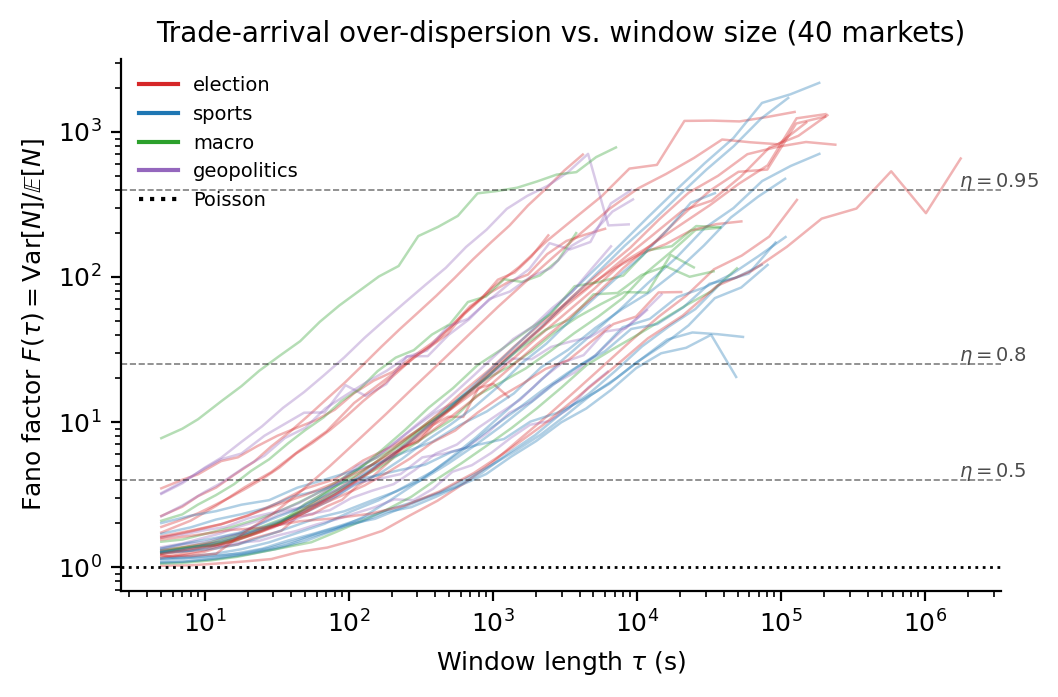
\includegraphics[width=0.92\linewidth]{figures/figure_1_fano_curves.png}
  \caption{Fano factor $F(\tau)=\mathrm{Var}[N(\tau)]/\mathbb{E}[N(\tau)]$
  vs.\ window length $\tau$ for each of 40 markets.  All curves rise
  sharply above the Poisson line $F=1$; many cross
  $F\!=\!1/(1\!-\!0.95)^2\!\approx\!400$. Curves are coloured by topic
  category.}
  \label{fig:fano}
\end{figure}

\paragraph{Headline numbers.} Across the 40 markets:
\begin{itemize}
  \item Inter-arrival CV: median $2.48$, IQR $[1.70, 3.31]$. The
        Kolmogorov-Smirnov test against the unit exponential rejects at
        $p<0.01$ in $40/40$ markets.
  \item Branching-ratio estimate $\hat\eta$ from
        Eq.~\ref{eq:eta}: median $0.933$, IQR $[0.91, 0.96]$, mean
        $0.925$. The minimum value is $0.766$ (the Trump-2024 tape,
        whose 3,500 trades span only $3.6$ hours of election night
        and so admit a Fano-curve estimate based on small bins).
  \item Trade-sign autocorrelation: $\rho(1)$ median $+0.19$,
        $\rho(5)$ median $+0.13$, $\rho(25)$ median $+0.06$. Across
        the full sample $\rho(\ell)$ stays above the $\pm 0.05$ band
        out to lag $\sim 50$ (Fig.~\ref{fig:sign}).
  \item Conspicuous-burst counts: the 60-second window mean for 4-sigma
        bursts is $318$; for 6-sigma bursts it is $201$. Across all
        markets we identify $12{,}738$ 4-sigma and $8{,}023$ 6-sigma
        burst windows in total. (We use these as descriptive
        complements to $\hat\eta$, not as cascades in any causal
        sense.)
\end{itemize}

\paragraph{Fano factor.} Figure~\ref{fig:fano} plots $F(\tau)$ for each
market. Every curve climbs from $F\!\sim\!1$ at $\tau\!\sim\!5$ s into a
plateau between $F\!\sim\!10$ and $F\!\sim\!10^3$ at the largest
$\tau$ admitted by the market's lifespan. The plateau values bracket
the eta-asymptote bands drawn in the figure: the typical
mid-volume market lies on or above the $\eta\!=\!0.8$ line, and many of
the long-lived political markets reach $\eta\!=\!0.95$. The Trump-2024
market is the visual outlier on the low side because its 3,500-trade
sample is dense in time and $F(\tau)$ has had no opportunity to
saturate at large $\tau$.

\begin{figure}[t]
  \centering
  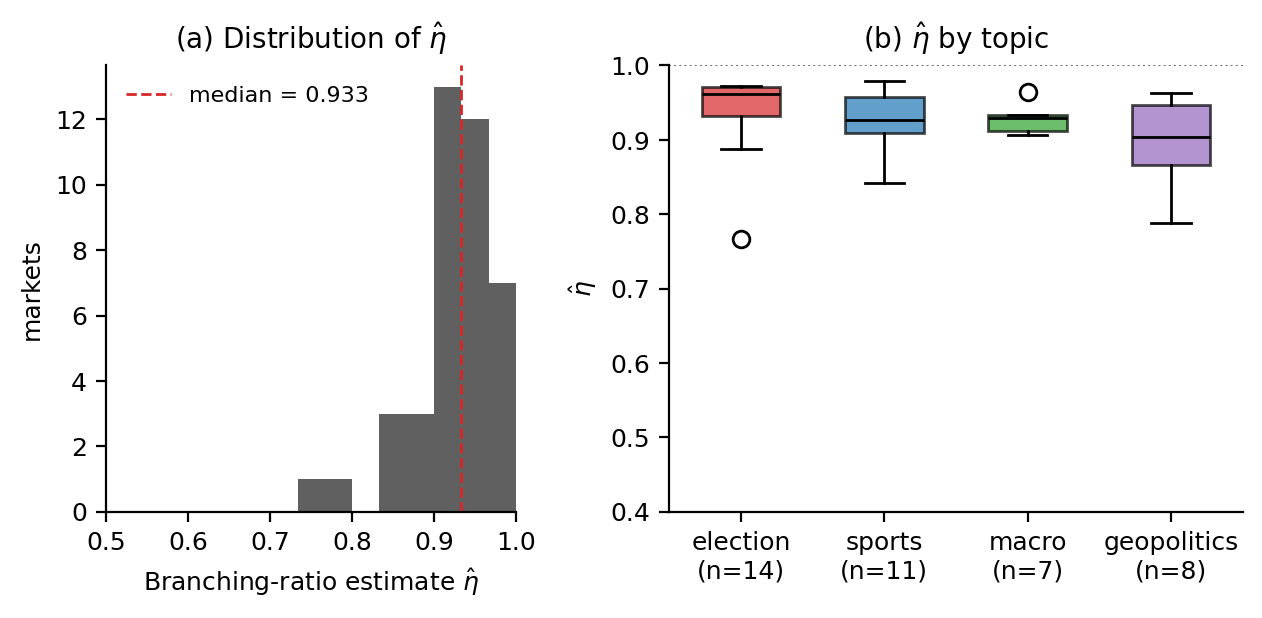
\includegraphics[width=0.95\linewidth]{figures/figure_2_eta_distribution.png}
  \caption{(a) Distribution of branching-ratio estimates $\hat\eta$
  across 40 markets; median $0.933$.  (b) $\hat\eta$ by topic.
  Election markets exhibit the highest typical reflexivity, with the
  Trump-2024 tape the lone outlier near $\hat\eta\!=\!0.77$.}
  \label{fig:eta}
\end{figure}

\paragraph{Branching ratio by topic.} Figure~\ref{fig:eta} shows the
distribution of $\hat\eta$ overall and by category. Election markets
have the tightest and highest distribution (median $0.962$). Sports
markets are next ($0.927$), followed by macro ($0.929$) and
geopolitics ($0.903$). The Trump-2024 outlier aside, all 40 markets
have $\hat\eta>0.76$.

\begin{figure}[t]
  \centering
  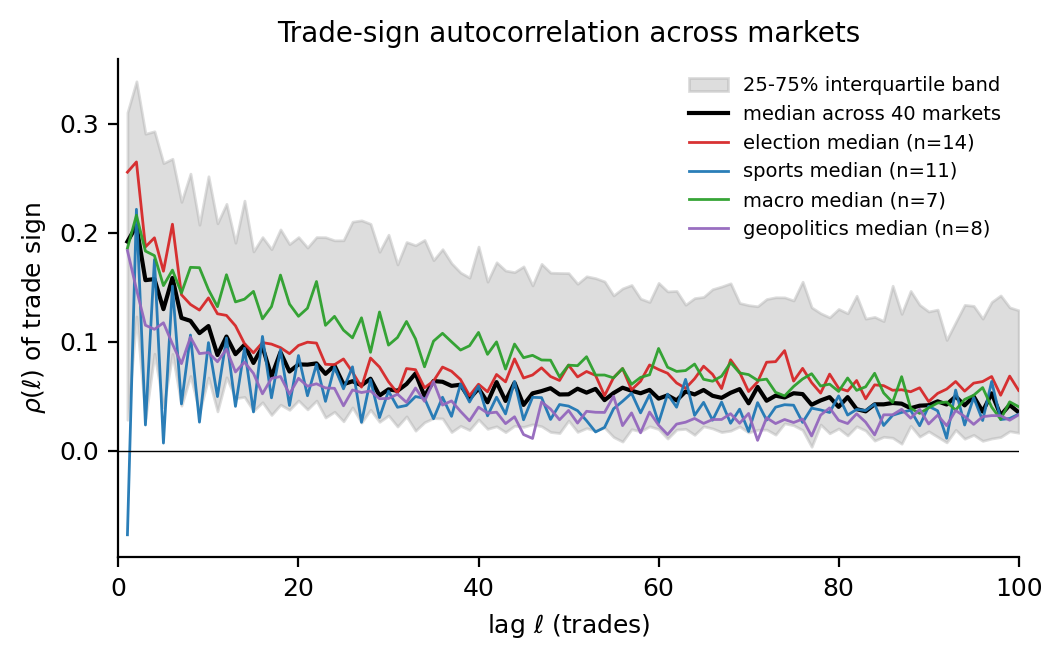
\includegraphics[width=0.85\linewidth]{figures/figure_3_sign_autocorr.png}
  \caption{Sample autocorrelation of the BUY/SELL taker-sign series
  $\rho(\ell)$ across 40 Polymarket order tapes. Black line is the
  market median; shaded band is the 25\,--\,75\% interquartile range.
  Coloured medians are by topic category.}
  \label{fig:sign}
\end{figure}

\paragraph{Sign autocorrelation.} Figure~\ref{fig:sign} shows the trade-sign
autocorrelation across markets. The aggregate median is positive at all
lags out to 100 trades and decays smoothly from $+0.19$ at lag 1 to
$+0.04$ at lag 100; election and macro markets have the highest medians
and the cleanest decay. Sports markets are the most striking exception:
several Super Bowl 2025 markets (Browns, Giants, Raiders, Panthers,
Titans) have $\rho(1)$ between $-0.17$ and $-0.27$. The sports-category
\emph{median} curve sits well below the aggregate, dipping below zero
inside the first 10 lags before recovering. This is consistent with
contrarian taker flow against a favourite that has just moved.

\begin{figure}[t]
  \centering
  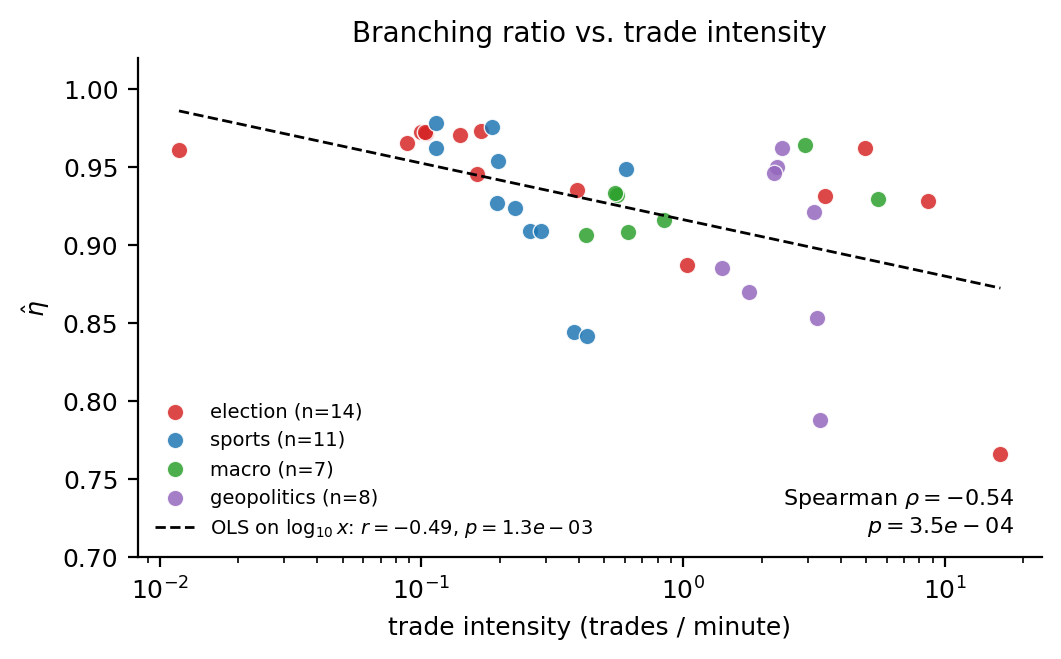
\includegraphics[width=0.85\linewidth]{figures/figure_4_intensity_vs_eta.png}
  \caption{Cross-section: branching-ratio estimate $\hat\eta$ against
  trade intensity. Higher-intensity markets have lower estimated
  branching ratios (Spearman $\rho=-0.54$, $p=3.5\times 10^{-4}$).}
  \label{fig:scatter}
\end{figure}

\paragraph{Cross-section: $\hat\eta$ versus activity.}
Figure~\ref{fig:scatter} plots $\hat\eta$ against trade intensity. The
Pearson correlation in log-intensity is $r=-0.49$ ($p=1.3\times
10^{-3}$); the Spearman rank correlation is $\rho=-0.54$
($p=3.5\times 10^{-4}$); the OLS slope in log-intensity is roughly
$-0.04$ per decade. The negative slope is striking because it is the
opposite sign to what \citet{hardiman2013critical} report for E-mini
S\&P futures, where within-day reflexivity rises during volume bursts
toward $\hat\eta\to 1$. We interpret the Polymarket pattern in
Section~\ref{sec:discussion}.

\paragraph{What about price impact?} Per-trade midprices on the data-API
are quoted to the nearest cent and saturate at the
0.99\,/\,0.01 boundary for many of our most-active markets near
close. The response function $R(\ell)$ is therefore numerically
ill-conditioned for our sample, and we do not report
it. \citet{dubach2026anatomy} has the higher-fidelity order-book data
required to study price impact properly.

\section{Discussion}\label{sec:discussion}

\paragraph{Why does $\hat\eta$ fall with intensity on Polymarket?}
The within-day equity finding of \citet{hardiman2013critical} is that
busier periods are more endogenous: more trades trigger more trades. Our
\emph{cross-market} finding is the opposite. We see three plausible
mechanisms, and our data cannot cleanly separate them.

(1) \emph{Bias of the Fano-based estimator.} Equation~\ref{eq:eta}
implicitly assumes an exponential triggering kernel, but
\citet{hardiman2013critical} explicitly show that empirical equity
kernels are heavy-tailed and that the moment-based $\hat\eta$ overshoots
in sparse data. Low-intensity markets in our sample have the same 3,500
trades stretched over weeks or months: their $F^\star$ is dominated by
a few unrepresentative bursts, inflating $\hat\eta$. We regard this
explanation as the most likely contributor.

(2) \emph{Taker-pool composition.} Low-volume markets attract a
narrower population of returning takers
\citep[whose trading is highly concentrated;][]{tsang2026anatomy}. A
narrower population mechanically produces more
trade-on-trade reactions per unit activity.

(3) \emph{Marketmaker behaviour.} High-intensity periods on Polymarket
coincide with denser MM quoting, which mechanically converts what
would be a triggered taker arrival into a passive fill against a
resting MM order. Our trade tape is taker-only, so MM-absorbed events
are filtered out; this filtering will be more aggressive at high
intensity, reducing the apparent branching ratio.

\paragraph{Are these information cascades?}  Strictly, a
\citet{bikhchandani1992theory} cascade requires that a rational agent
ignore their private signal in favour of the observed action of others.
Our measurements speak to the necessary statistical signatures
(over-dispersed arrivals, positive sign autocorrelation,
trade-on-trade triggering) but not to the agents' epistemic states.
What we can claim is that \emph{any} model in which Polymarket prices
result from independent draws of private information is
straightforwardly refuted: trade flow is far too clustered.

\paragraph{What about calibration?} Polymarket markets resolve almost
exactly to their final-day midprice in our sample (median 24-hour
Brier $\sim 10^{-6}$). Strong endogeneity in the trade-arrival
process is therefore compatible with accurate aggregate prices,
just as it is in equity index futures
\citep{hardiman2013critical}. Reflexivity and calibration are
distinct phenomena.

\section{Limitations}\label{sec:limitations}

\paragraph{Trade-direction inference.} \citet{dubach2026anatomy}
documents that BUY/SELL direction inferred from public order-book
updates agrees with on-chain truth in only $\sim$59\% of cases. We
read the side field directly from the \texttt{data-api}, which we
believe is on-chain-derived (the entries are taker-only), so this
caveat does not directly affect our $\rho(\ell)$ estimates, but we
have not independently verified it; a paper that wanted to cite the
sign-autocorrelation numbers in production should cross-check against
the on-chain logs Dubach uses.

\paragraph{Sample cap.} The \texttt{data-api} hard-caps offset at
$\sim$3,500. For high-volume markets such as the Trump-2024 contract
this restricts us to the final hours of trading. Our $\hat\eta$
estimates are therefore for the cascade-prone tail of each market,
not its life as a whole.

\paragraph{Moment estimator.} The Fano-based $\hat\eta$ is a
diagnostic, not a structural MLE. \citet{hardiman2013critical}
calibrate the moment estimator on simulated Hawkes processes and
report that its bias toward $\hat\eta\to 1$ becomes severe for
sample sizes below $\sim 10{,}000$; our 3,500-trade samples sit
inside that regime, and the absolute level of our $\hat\eta$ should be
interpreted with caution. The within-sample \emph{ordering} of
markets is more robust than the level.

\paragraph{Resolution.} The 12-hour CLOB price history we use for
calibration cannot be refined further on closed markets via the public
endpoint; intraday price dynamics around the events of interest
(Biden dropout, debate windows, Fed meetings) are not analysable from
the public CLOB feed and would require subscription
order-book data.

\paragraph{Category labels.} We classify markets by keyword and the
counts in each cell are small ($n\!=\!7$ for macro, $n\!=\!8$ for
geopolitics). The category comparisons should be read as suggestive,
not inferential.

\section{Conclusion}

Polymarket trade tapes are very far from Poisson and exhibit
branching-ratio estimates close to the values reported for equity
index futures. The order of the markets by reflexivity is interpretable
(elections and macroeconomic markets the most cascade-like; sports
markets occasionally contrarian), and the cross-market relationship
between activity and apparent endogeneity is the opposite of the
within-day equity pattern in the same diagnostic. None of this implies
that prediction markets are bad at aggregating information: our
markets calibrate to outcome at the percent level by close. It does
imply that the path by which a market arrives at its closing price is
dominated by trade-on-trade triggering rather than by a sequence of
independent informational arrivals\,---\,which is exactly what one
would expect from the cascade theory of
\citet{bikhchandani1992theory} applied to a continuously-quoted
order book.

\paragraph{Reproducibility.} The two python scripts in
\texttt{scripts/} produce every number in this paper from the public
Polymarket endpoints. With \texttt{requirements.txt} pinned, the
full pipeline runs in roughly 10 minutes on a laptop and writes a
21 MB working directory.

{
\small
\bibliographystyle{plainnat}
\bibliography{references}
}

\end{document}
